\documentclass{beamer}
\usepackage[utf8]{inputenc}

\usetheme{Madrid}
\usecolortheme{default}
\usepackage{amsmath,amssymb,amsfonts,amsthm}
\usepackage{txfonts}
\usepackage{multicol}
\usepackage{tkz-euclide}
\usepackage{listings}
\usepackage{adjustbox}
\usepackage{array}
\usepackage{tabularx}
\usepackage{gvv}
\usepackage{lmodern}
\usepackage{circuitikz}
\usepackage{tikz}
\usepackage{graphicx}
\usepackage{hyperref}

\setbeamertemplate{page number in head/foot}[totalframenumber]

\usepackage{tcolorbox}
\tcbuselibrary{minted,breakable,xparse,skins}



\definecolor{bg}{gray}{0.95}
\DeclareTCBListing{mintedbox}{O{}m!O{}}{%
  breakable=true,
  listing engine=minted,
  listing only,
  minted language=#2,
  minted style=default,
  minted options={%
    linenos,
    gobble=0,
    breaklines=true,
    breakafter=,,
    fontsize=\small,
    numbersep=8pt,
    #1},
  boxsep=0pt,
  left skip=0pt,
  right skip=0pt,
  left=25pt,
  right=0pt,
  top=3pt,
  bottom=3pt,
  arc=5pt,
  leftrule=0pt,
  rightrule=0pt,
  bottomrule=2pt,
  toprule=2pt,
  colback=bg,
  colframe=orange!70,
  enhanced,
  overlay={%
    \begin{tcbclipinterior}
    \fill[orange!20!white] (frame.south west) rectangle ([xshift=20pt]frame.north west);
    \end{tcbclipinterior}},
  #3,
}
\lstset{
    language=C,
    basicstyle=\ttfamily\small,
    keywordstyle=\color{blue},
    stringstyle=\color{orange},
    commentstyle=\color{green!60!black},
    numbers=left,
    numberstyle=\tiny\color{gray},
    breaklines=true,
    showstringspaces=false,
}
%------------------------------------------------------------
%This block of code defines the information to appear in the
%Title page
\title %optional
{5.2.7}
\date{September 20,2025}
%\subtitle{A short story}

\author % (optional)
{Aditya Appana - EE25BTECH11004}



\begin{document}


\frame{\titlepage}
\begin{frame}{Question}
Solve the following system of linear equations.\\
$$\frac{3}{2}x + \frac{5}{3}y= 7$$
$$9x-10y=14$$
\end{frame}



\begin{frame}[fragile]
    \frametitle{Solution}
Organizing the given equations into an augmented matrix:
\begin{align}
\myvec{\frac{3}{2}& \frac{5}{3} & 7 \\ 9 & -10 & 14}
\end{align}\\
Performing row operations:
\begin{align}
\myvec{\frac{3}{2}& \frac{5}{3} & 7 \\ 9 & -10 & 14} \xrightarrow{\text{R_2 \rightarrow $R_2- 6R_1$}}\\
 \myvec{\frac{3}{2}& \frac{5}{3} & 7 \\ 0 & -20 & -28}  \xrightarrow{\text{R_1 \rightarrow $R_1+ \frac{1}{12}R_2$}} \\
 \myvec{\frac{3}{2}& 0 & \frac{14}{3} \\ 0 & -20 & -28} 
\end{align}
Solving, we get the solution as:
\begin{align}
\vec{x}= \myvec{\frac{28}{9}\\\frac{7}{5}}
\end{align}

\end{frame}

\begin{frame}[fragile]
    \frametitle{Python Code}

    \begin{lstlisting}
import numpy as np
import numpy.linalg 
import matplotlib.pyplot as plt

answer = numpy.linalg.solve([[3/2, 5/3],[9,-10]], [7,14])

answer[0] = round(answer[0],2)
answer[1] = round(answer[1],2)
print(answer)
\end{lstlisting} 
\end{frame}

\begin{frame}[fragile]
    \frametitle{Python Code}

    \begin{lstlisting}


fig = plt.figure(figsize =(6,6))
ax = fig.add_subplot(111)

X = np.linspace(-20,20,2)

Y1 = -0.6*(1.5*X-7)
Y2 = 0.1*(9*X-14)

ax.plot(X, Y1, label='Line 1')
ax.plot(X, Y2, label='Line 2')
ax.scatter(answer[0], answer[1], label=f'({answer[0]}, {answer[1]})')
ax.grid(True)
ax.legend()
plt.show()

    \end{lstlisting}
\end{frame}

\begin{frame}[fragile]
\frametitle{Plot}

\begin{figure}[H]
    \centering
    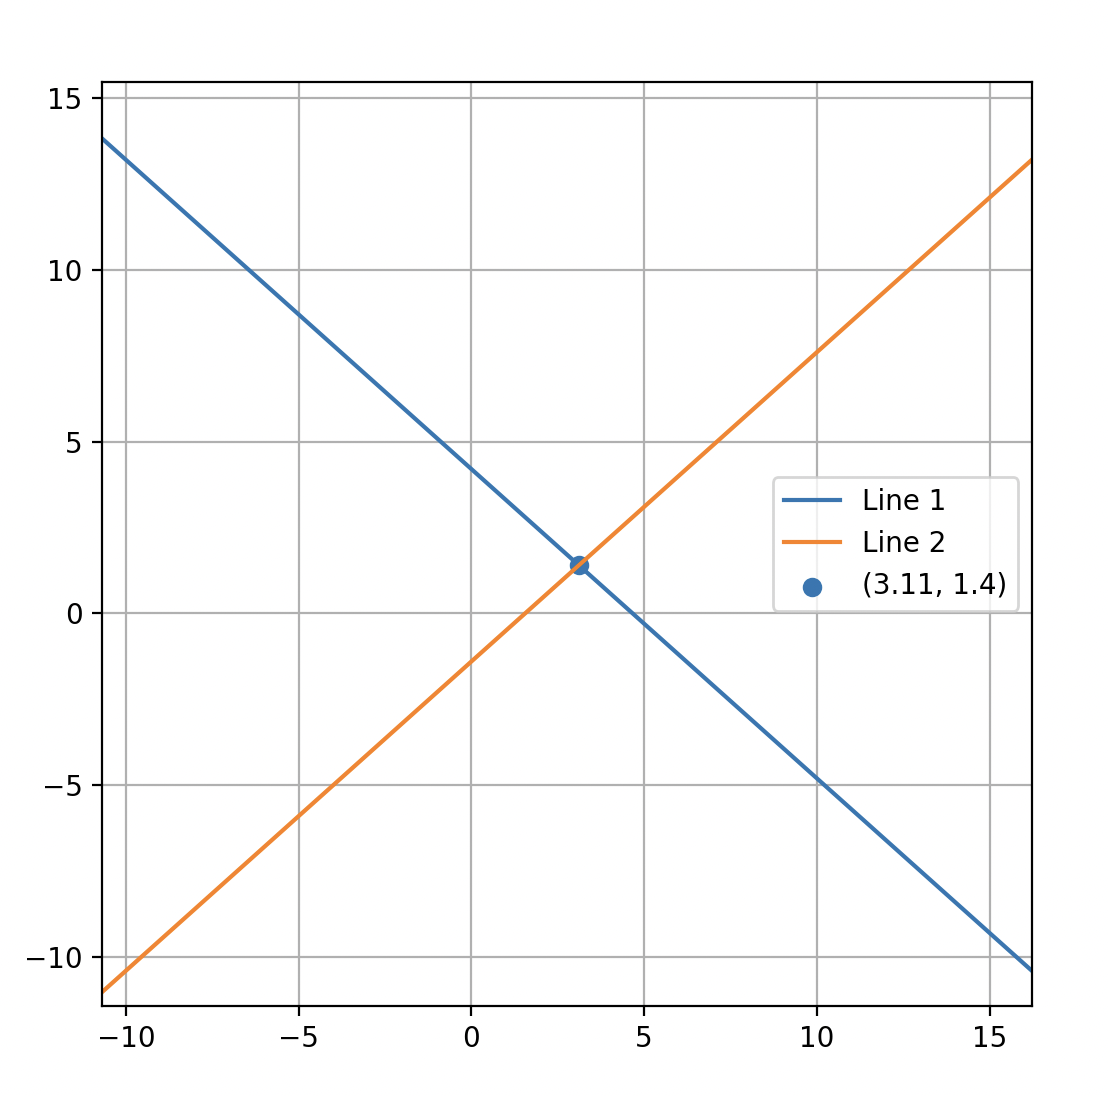
\includegraphics[width=0.7\columnwidth]{Figs/527.png}
    \caption{Plot}
    \label{fig:placeholder}
\end{figure}

\end{frame}
\end{document}